\documentclass[11pt,a4paper,twocolumn]{article}

\usepackage[T1]{fontenc}
\usepackage[utf8]{inputenc}
\usepackage[left=0.5in,top=0.5in,right=0.5in,bottom=0.5in,nohead,nofoot]{geometry}
\usepackage{graphicx}
\usepackage{url}
\usepackage{float}
\usepackage[today,revrange,nofancy]{svninfo}
\graphicspath{ {./design_brief_contents/System_Design/} }
\svnInfo $Id: design_brief.tex 2489 2019-02-13 11:08:51Z jbri2 $

\renewcommand\abstractname{Executive Summary}

\title{Design Brief: Group 2}
\author{
   Aidan Cauchi,
   Matthew Vella,
   Neil Vassallo,
   Peter Galea St. John
   }
\date{\svnMaxToday, Document v.\svnInfoMaxRevision}

\begin{document}

\maketitle

\abstract{%
  Everyone likes to have fun! And everyone remembers a certain game in particular.
Reminiscing about the time we were kids, arcade games gave us the perfect opportunity to have fun
whilst competing with our friends.
Given the opportunity to work on this project, as well as all the good memories the team made playing
such games, they have decided to make an arcade classic that they all loved, the basketball hoop game.
The player to score the most wins!
   }

\section{Introduction}
\par{The team members have chosen this game as they all love games and it would be interesting to create their own game, with the ARM MDK. Furthermore, while the project does seem challenging since the team is new to the concepts mentioned, 
it also seems manageable enough such that the members don't end up feeling overwhelmed while managing other projects as well.}
\newline

\par{The ARM MDK would be set up to a wooden architecture, where the components needed would be attached to it.
The player, after interacting with the menu system, would try to shoot the ball in the hoop, and gain points if succeeding in doing so. 
The ball would return back to the player and they will try to get more points until they run out of time. Once this happens, the final score will then then be saved onto persistent storage to keep track of "highscores".}
\newline


\par{This document is divided into 3 other sections.
Firstly, there is the System Design, where the descriptions of logic, architecture, tools, and explanation of the actual implementation of the project are found.
Secondly, the Management section involves how the team will work together, and the development methodology they will adopt. 
Finally, the Closure section contains a small recap and members' expectations with the project going forward.}


\section{System Design}
This section contains the implementation details of the project.

\subsection{List of components}
The team will be making use of the following components:
\begin{itemize}
	\item Joystick
	\item IR Sensor Switch E18-D80NK-N
	\item Hitachi HD44780-based 2-line text LCD display
	\item LEDs
\end{itemize}

\subsection{Functional Requirements}
The following table shows how the team intends to meet the project requirements:


\vspace{1cm}

\resizebox{\columnwidth}{!}{%
\renewcommand{\arraystretch}{2}
\begin{tabular}{l|p{0.5\columnwidth}}
 Requirement&  How it's addressed\\
\hline
 (F.1) – Real time System&  Interrupt based system reacting to the ball going through hoop. Also works on timer interrups generated every second.\\
 (F.2) – Digital Input&  Joystick, IR Sensor Switch E18-D80NK-N.\\
 (F.3) – Digital Output&  Hitachi HD44780-based 2-line text LCD display, LED. \\
 (F.4) – External Peripheral&  Hitachi HD44780-based 2-line text LCD display, LED and the  IR Sensor Switch E18-D80NK-N.\\
 (F.5) – Well defined states&  To be tackled with software.\\
 (F.6) – Persistent Storage&  On board EEPROM.\\
 (F.7) – Error reporting&  LCD for error reporting. \\
 (F.8) – Robust System&  Tacked with software. 
\end{tabular}
}

\subsection{Joystick}
This will be used to control the menu outputted on the LCD screen. The user will be able to switch through the menu options and press the joystick when s/he wants to make a choice.

\subsection{IR Sensor Switch E18-D80NK-N}
This sensor will be used to count the amount of times the user manages to score a point. It create an interrupt every time it detects a change in state, i.e. when a ball passes it, the sensor will go high and low again which will prompt the microcontroller to increment the score.

\subsection{LED Lights}
These will switch on and flash when a game is started and when a goal is scored.

\subsection{Hitachi HD44780-based 2-line text LCD display}
The LCD screen will be used to display the menu. In it the user can chose to start a new game, view scores and change game settings. Furthermore, it is used to display the details of an on going game i.e the current score and the time left.

\subsection{Gameplay Loop}
Figure \ref{flow} shows the flowchart for the main gameplay loop, where the majority of the logic of the game resides.

\begin{figure}[!ht]
	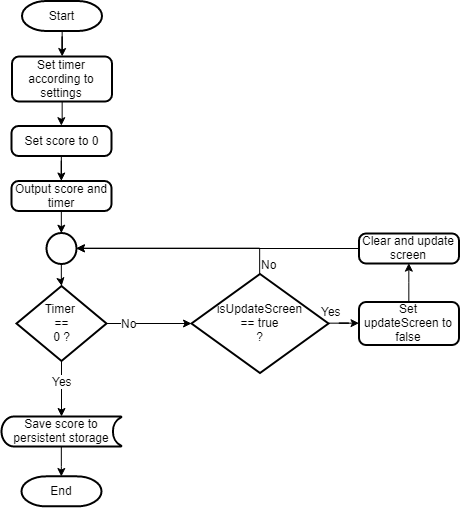
\includegraphics[width=0.5\textwidth]{InGameLoopFC.png}
\caption{Flowchart of the main gameplay loop.}
\label{flow}
\end{figure}

Alongside the logic in Figure \ref{flow}, the game makes use of 2 interrupt handlers. On the falling edge of the IR Sensor, an interrupt is generated which increases the total score by 1 and sets the updateScreen flag to true. Similarly, the timer generates an interrupt every second, which decreases the total time left and also sets the updateScreenFlag to true. When this is detected, the main program updates the screen and sets the flag to false.


Another thing to note is that only the last score is saved rather than the top score. This is because since due to testing scores were being generated manually by messing with the sensor, the team didn't want the highest score to be an unfair one. Furthermore, this helps the team further ensure that the score saving is indeed working, as it is updated after every game and thus testing wouldn't take a lot of effort.

\subsection{Menu Loop}
Figure \ref{men} shows the loop of the main menu. The first state leads to the main gameplay loop. The second state allows the user the change the time limit of the game from a preset number of options (15, 30, 45, 60). Finally, the third state allows the user to view to most recently saved score.

\begin{figure}[!ht]
	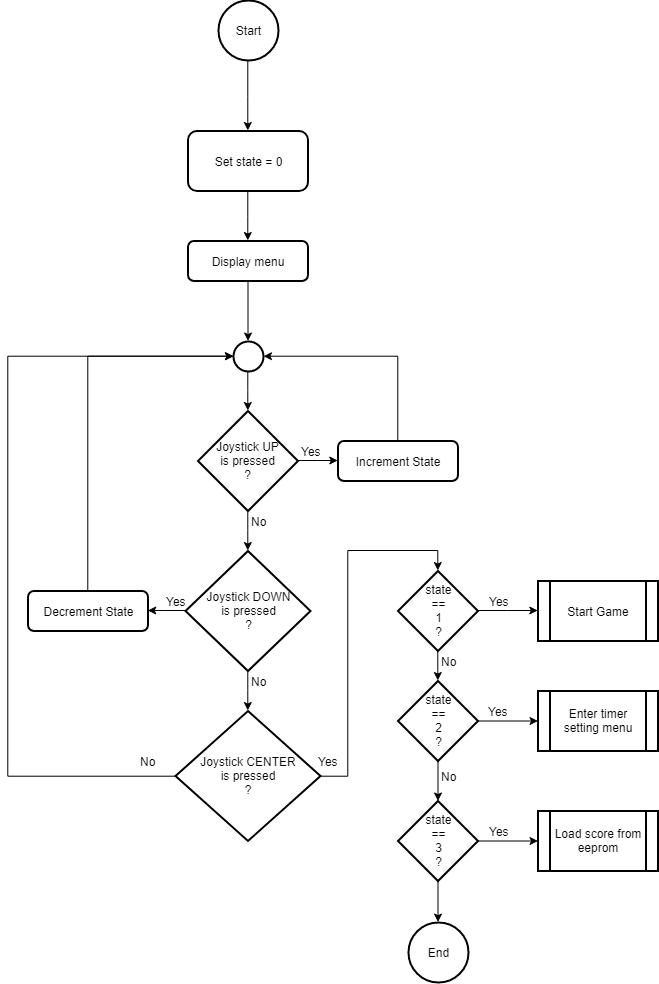
\includegraphics[width=0.5\textwidth]{menuLoop.png}
\caption{Flowchart of the main menu loop.}\label{men}
\label{flow}
\end{figure}

\subsection{Physical Design}
Figures \ref{physical1} and \ref{physical2} contain the diagrams related to the physical model. The model is made of plywood (thick but lightweight) and is 70cm by 55cm and the back court is 55cm by 50cm. Finally, the board is fitted at the end of the ramp as this reduces most of the wiring issues.

\begin{figure}[!htb]
	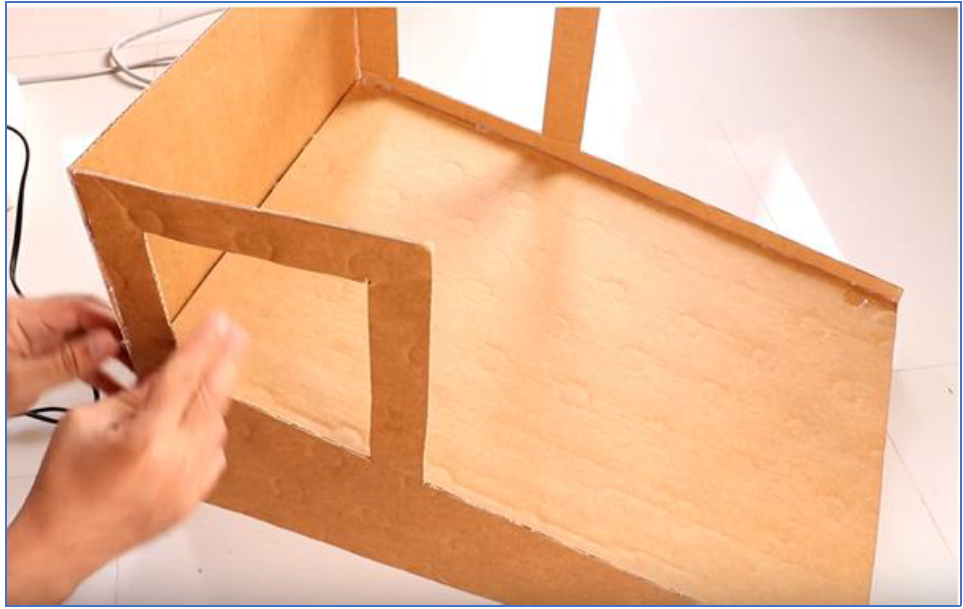
\includegraphics[width=0.5\textwidth]{MeasurementsPic2.png}
\caption{Approximation of how the model will look \cite{model}}
\label{physical1}
\end{figure}

\begin{figure}[!htb]
	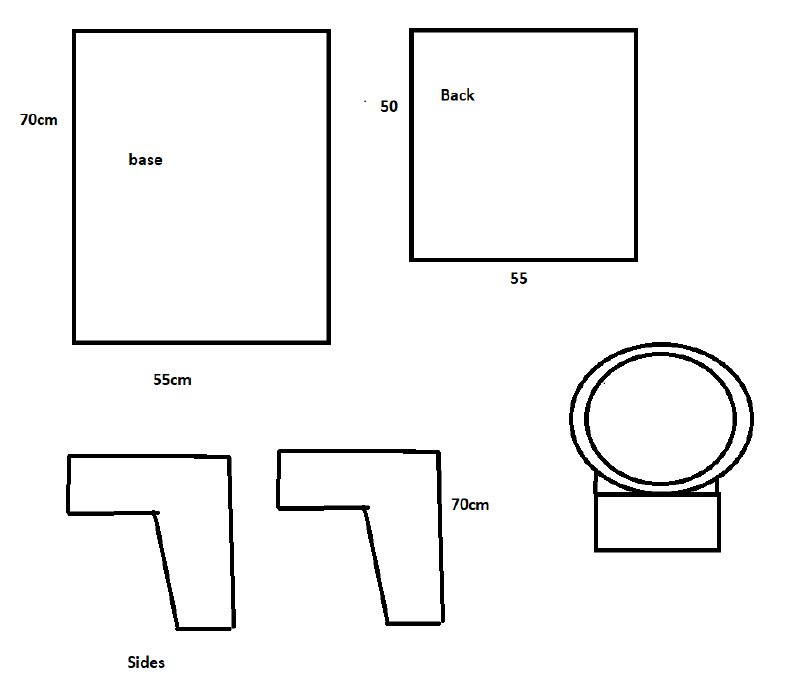
\includegraphics[width=0.5\textwidth]{MeasurementsPic1.png}
\caption{Top-Down Designs}
\label{physical2}
\end{figure}

\newpage
\section{Management}
\par{Being four people in the group, it was seen ideal to split the group up; Matthew and Peter will work mostly on hardware while Aidan and Neil will work mostly on software. However, this will not be strictly enforced so that all members will get a chance to work on all aspects of the project.}
\newline

\par{After the initial meeting, the team agreed to proceed with the Agile Software Development approach. This approach will allow them to work in a flexible manner. As the technology is new to all members, it is essential that there is some space to allow requirements to change as necessary without severely halting the progress of the project \cite{agileDev}. However, some key requirements were still noted:
\begin{itemize}
	\item Interfacing with LCD.
	\item Wiring/integrating components.
	\item Testing.
	\item Lighting LEDs.
	\item Joystick programming.
	\item Main menu programming.
	\item  In-game programming.
	\item Score persistence.
\end{itemize}
The prioritisation of these requirements will be discussed during the meetings as the team starts to get a better understanding of the technology.
}
\newline

\par{As a result of choosing this methodology, some ground rules needed to be set: The team is to meet every Thursday at 12/12:30. An agenda detailing the points of discussion for the next meeting will be uploaded by a member on SVN before the next meeting. On the agenda, a member is chosen to be the minute-taker for the next meeting. After a meeting has concluded, the minute-taker will compile the minutes using the template provided on SVN and then upload said minutes. The minutes are to contain what was said in the meeting as well as the work assigned to each member for the next meeting. Once uploaded, the minutes and agendas shouldn't be changed, however some exceptions will be permitted if some information was overlooked, especially in the beginning few weeks as the team gets used to the system. The members taking the minutes and agendas will be rotated every week so that everyone will get a chance to contribute from a managerial perspective. Finally, all the minutes and agendas will be written using Latex and the provided templates.}
\newline

\par{With respect to the project itself, detailed goals will be listed during each meeting. Since most members of the group have no experience using this technology, it was found to be better to plan specific requirements as the project develops and as the team learns more during the lectures. The Keil uVision IDE will be used to code the implementation. Alongside this, the team will make use of Doxygen to ensure proper and consistent documentation of code. Moreover, SVN will be used to track changes to the project and share files between the team members. Facebook's Messenger will be used for informal communication between the members and for providing online help. Finally, the University email will be used to formally remind each member before each meeting.}

\section{Closure}

\par{To recap, all the work was divided between all members of the group. Minute-taking and the writing
of agendas are to be done by weekly-rotations between group members and detailed goals are
listed during each meeting.
}
\newline
\par{By evaluating the group performance weekly, the team feels that they're on the right track and
moving forward as a group. The project seems very interesting and all members are keen to learn
and challenge themselves.}
\newline
\par{By the end of this project, they hope to have a much greater understanding of coding low level
microcontrollers, make better use of SVN and enhance their group work skills, especially through the
Agile Development Cycle.}

\bibliographystyle{ieeetr}
\bibliography{references}

\end{document}
